\documentclass[border=10pt]{standalone}
\usepackage{tikz}
\usepackage{xcolor}
\usepackage{amsmath}

\begin{document}
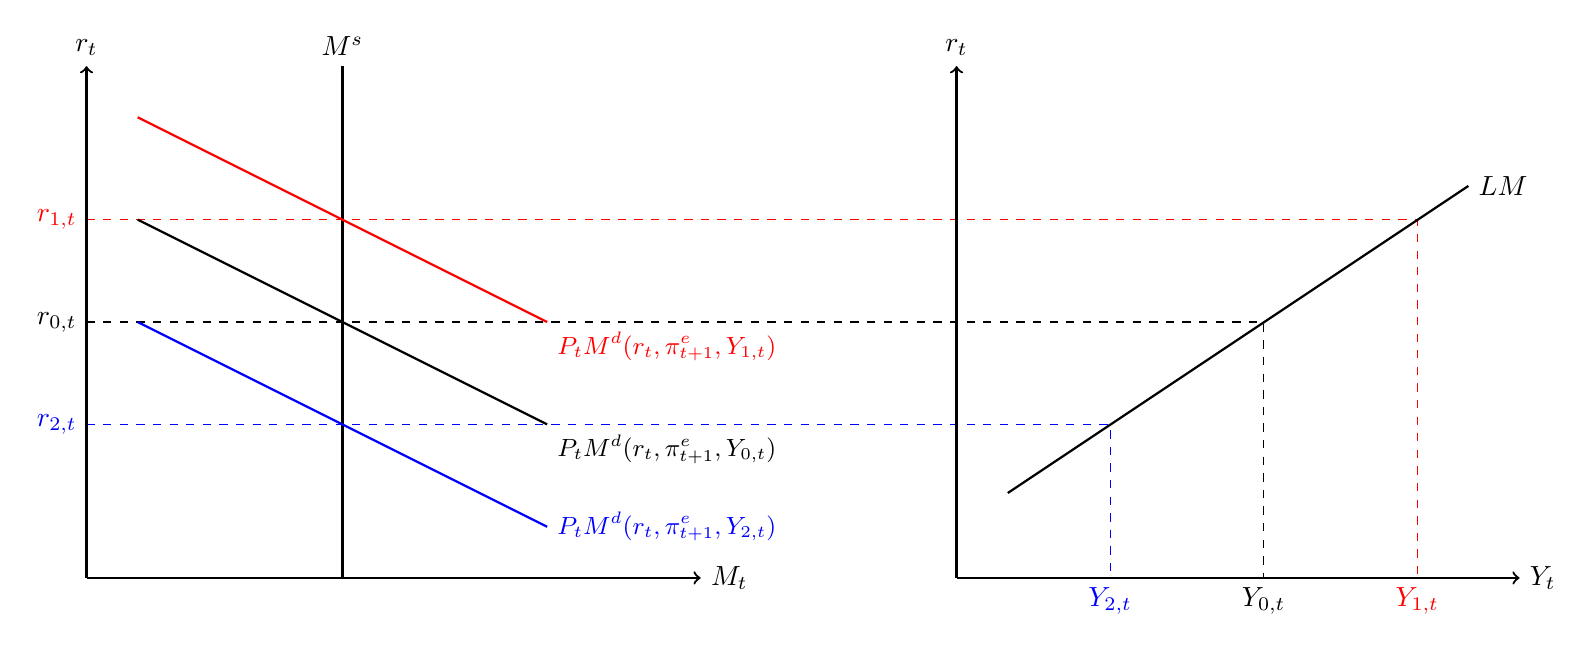
\begin{tikzpicture}[scale=1.3]

    % ==========================================
    % CONNECTING DASHED LINES (Drawn first to stay in background)
    % ==========================================
    
    % High interest rate (r1) -> High output (Y1)
    \draw[dashed, red] (0, 3.5) -- (13, 3.5) -- (13, 0);
    
    % Equilibrium interest rate (r0) -> Medium output (Y0)
    \draw[dashed, black] (0, 2.5) -- (11.5, 2.5) -- (11.5, 0);
    
    % Low interest rate (r2) -> Low output (Y2)
    \draw[dashed, blue] (0, 1.5) -- (10, 1.5) -- (10, 0);

    % ==========================================
    % LEFT GRAPH: Money Market
    % ==========================================
    
    % Axes
    \draw[thick, ->] (0,0) -- (6,0) node[right] {$M_t$};
    \draw[thick, ->] (0,0) -- (0,5) node[above] {$r_t$};

    % Money Supply (M^s) vertical line
    \draw[thick] (2.5, 0) -- (2.5, 5) node[above] {$M^s$};

    % Money Demand Curves
    % Red (Highest income Y_1)
    \draw[thick, red] (0.5, 4.5) -- (4.5, 2.5) node[below right, font=\small] {$P_t M^d(r_t, \pi_{t+1}^e, Y_{1,t})$};
    
    % Black (Middle income Y_0)
    \draw[thick, black] (0.5, 3.5) -- (4.5, 1.5) node[below right, font=\small] {$P_t M^d(r_t, \pi_{t+1}^e, Y_{0,t})$};
    
    % Blue (Lowest income Y_2)
    \draw[thick, blue] (0.5, 2.5) -- (4.5, 0.5) node[right, font=\small] {$P_t M^d(r_t, \pi_{t+1}^e, Y_{2,t})$};

    % Y-axis Labels
    \node[left, red] at (0, 3.5) {$r_{1,t}$};
    \node[left, black] at (0, 2.5) {$r_{0,t}$};
    \node[left, blue] at (0, 1.5) {$r_{2,t}$};

    % ==========================================
    % RIGHT GRAPH: LM Curve Derivation
    % ==========================================
    
    % Shift coordinate system right by 8.5cm for the right graph
    \begin{scope}[xshift=8.5cm]
        % Axes
        \draw[thick, ->] (0,0) -- (5.5,0) node[right] {$Y_t$};
        \draw[thick, ->] (0,0) -- (0,5) node[above] {$r_t$};

        % LM Curve 
        \draw[thick] (0.5, 0.83) -- (5, 3.83) node[right] {$LM$};

        % X-axis Labels
        \node[below, blue] at (1.5, 0) {$Y_{2,t}$};
        \node[below, black] at (3.0, 0) {$Y_{0,t}$};
        \node[below, red] at (4.5, 0) {$Y_{1,t}$};
    \end{scope}

\end{tikzpicture}
\end{document}